\chapter{Server Side Template Injection (SSTI)}
\section{Definition}
A server-side template injection occurs when an attacker is able to use native
template syntax to inject a malicious payload into a template, which is then
executed server-side.a

Template engines are designed to generate web pages by combining fixed
templates with volatile data. Server-side template injection attacks can occur
when user input is concatenated directly into a template, rather than passed in
as data. This allows attackers to inject arbitrary template directives in order
to manipulate the template engine, often enabling them to take complete control
of the server.a

An example of vulnerable code see the following one:
\begin{verbatim}
output = $twig->render("Dear " . $_GET['name']);
\end{verbatim}

In the previous example part of the template itself is being dynamically
generated using the GET parameter name. As template syntax is evaluated
server-side, this potentially allows an attacker to place a server-side
template injection payload inside the name parameter as follows:

\begin{verbatim}
http://vulnerable-website.com/?name={{bad-stuff-here}}
\end{verbatim}

\section{Constructing a server-side template injection attack}
\subsection{Detect}
As with any vulnerability, the first step towards exploitation is being able to
find it. Perhaps the simplest initial approach is to try fuzzing the template
by injecting a sequence of special characters commonly used in template
expressions, such as the polyglot \verb+${{<%[%'"}}%\+.
In order to check if the server is vulnerable you should spot the differences
between the response with regular data on the parameter and the given payload.

If an error is thrown it will be quiet easy to figure out that the server is
vulnerable and even which engine is running. But you could also find a
vulnerable server if you were expecting it to reflect the given payload and it
is not being reflected or if there are some missing chars in the response.

\textbf{Plaintext context}
The given input is being rendered and reflected into the response. This is
easily mistaken for a simple XSS vulnerability, but it's easy to differentiate
if you try to set mathematical operations within a template expression:

\begin{verbatim}
{{7*7}}
${7*7}
<%= 7*7 %>
${{7*7}}
#{7*7}
\end{verbatim}


\textbf{Code context}
In these cases the user input is being placed within a template expression:
\begin{verbatim}
engine.render("Hello {{"+greeting+"}}", data)
\end{verbatim}

The URL access that page could be similar to:\\
\verb+http://vulnerable-website.com/?greeting=data.username+

If you change the greeting parameter for a different value the response won't
contain the username, but if you access something like:\\
\verb+http://vulnerable-website.com/?greeting=data.username}}hello+

then, the response will contain the username (if the closing template
expression chars were \verb+}}+).

If an error is thrown during these test, it will be easier to find that the
server is vulnerable.



\subsection{Identify}
Once you have detected the template injection potential, the next step is to
identify the template engine.

Although there are a huge number of templating languages, many of them use very
similar syntax that is specifically chosen not to clash with HTML characters.
If you are lucky the server will be printing the errors and you will be able to
find the engine used inside the errors. Some possible payloads that may cause
errors:

\begin{verbatim}
${}
${7/0}
${foobar}
${7*7}

{{}}
{{7/0}}
{{foobar}}
{{7*7}}

<%= %>
<%= 7/0 %>
<%= foobar %>
``
\end{verbatim}
Otherwise, you'll need to manually test different language-specific payloads
and study how they are interpreted by the template engine. A common way of
doing this is to inject arbitrary mathematical operations using syntax from
different template engines. You can then observe whether they are successfully
evaluated. To help with this process, you can use a decision tree similar to
the following

\begin{figure}
  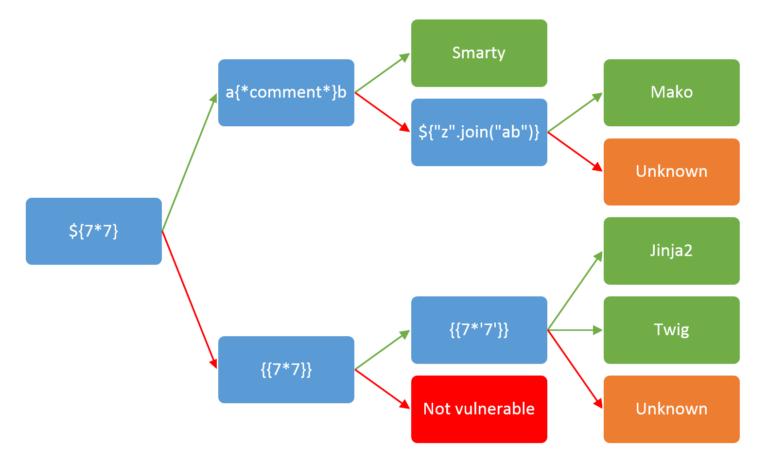
\includegraphics[width=\linewidth]{web/ssti/images/server_side_template_injection.png}
  \caption{decision tree}
  \label{fig:decision_tree}
\end{figure}

This diagram is not complet. For example  Tornado template engine has payload
in form of \verb+{{os.system('whoami')}}+\ldots

In addition to the above diagram, try the following approaches to recognize the
technology: 
\begin{itemize}
\item    Check verbose errors for technology names. Sometimes just copying the error in Google search can provide with a straight answer regarding the underlying technology used
\item    Check for extensions. For example, \verb+.jsp+ extensions are
    associated with Java. When dealing with Java, we may be facing an
    expression \verb+language/OGNL+ injection vulnerability instead of
    traditional SSTI
\item    Send expressions with unclosed curly brackets to see if verbose errors
    are generated. Do not try this approach on production systems, as it may
    crash the webserver.
\end{itemize}


\subsection{Exploit}
\textbf{Read}
The first step after finding template injection and identifying the template
engine is to read the documentation. Key areas of interest are:
\begin{itemize}
    \item 'For Template Authors' sections covering basic syntax.
    \item 'Security Considerations' - chances are whoever developed the app you're testing didn't read this, and it may contain some useful hints.
    \item Lists of builtin methods, functions, filters, and variables.
    \item Lists of extensions/plugins - some may be enabled by default.
\end{itemize}
\textbf{Explore}
Assuming no exploits have presented themselves, the next step is to explore the
environment to find out exactly what you have access to. You can expect to find
both default objects provided by the template engine, and application-specific
objects passed in to the template by the developer. Many template systems
expose a 'self' or namespace object containing everything in scope, and an
idiomatic way to list an object's attributes and methods.

If there's no builtin self object you're going to have to bruteforce variable
names using SecList and Intruder's wordlist collection.

Developer-supplied objects are particularly likely to contain sensitive
information, and may vary between different templates within an application, so
this process should ideally be applied to every distinct template
individually.

\subsection{Attack}
At this point you should have a firm idea of the attack surface available to
you and be able to proceed with traditional security audit techniques,
reviewing each function for exploitable vulnerabilities. It's important to
approach this in the context of the wider application - some functions can be
used to exploit application-specific features. The examples to follow will use
template injection to trigger arbitrary object creation, arbitrary file
read/write, remote file include, information disclosure and privilege
escalation vulnerabilities.

\section{Tools}
\begin{itemize}
    \item \url{https://github.com/epinna/tplmap}
    \item  word list from secList: \verb+SecLists/Fuzzing/template-engines-special-vars.txt+
    \item
        \url{https://github.com/carlospolop/Auto_Wordlists/blob/main/wordlists/ssti.txt}
\end{itemize}

\subsection{Tplmap}

\begin{verbatim}
./tplmap.py -u 'http://<TARGET IP>:<PORT>' -d <PARAM NAME>=toto
\end{verbatim}


\begin{verbatim}
/tplmap.py -u 'http://<TARGET IP>:<PORT>' -d <PARAM NAME>=toto --os-shell
\end{verbatim}


\subsection{links}
\url{https://book.hacktricks.xyz/pentesting-web/ssti-server-side-template-injection}
\url{https://github.com/swisskyrepo/PayloadsAllTheThings/blob/master/Server%20Side%20Template%20Injection/README.md}
